
Провести полное исследование функции и построить график функции:

\[
    y = \frac{x^4}{(x+1)^3}
\]

1. Найдем область определения функции: $D(x) = (- \infty,-1) \cup (-1, + \infty)$

2. Четноть, нечетность, периодичность.

Четность: проверим $y(-x) = \frac{x^4}{(-x+1)^3}$, то есть $y(-x) \neq y(x)$. Значит функция не четна.
Нечетность: так как $y(-x) \neq -y(x)$ функция не нечетна.
Так как в состав функции не входят периодичные функции - функция непериодична.

3. Непрерывность: 
Функция элементарная, значит непрерывна на своей области определения, осталось проверить характер разрыва в точке -1:
\[
    \lim_{x \rightarrow -1-0}y(x) = \frac{1}{-0^3} = - \infty 
\]
\[
    \lim_{x \rightarrow -1+0}y(x) = \frac{1}{+0^3} = + \infty 
\]

Значит, -1 - точка разрыва второго рода.

4. Асимптоты: 
Так как при $x = -1$ функция терпит разрыв второго рода, прямая $x = -1$ является вертикальной асимптотой.

Найдем наклонные асимптоты: пусть она имеет вид: $y = kx +b$, тогда

\[
    k = \lim_{x \rightarrow \infty}\frac{x^4}{x \cdot (x+1)^3} = 1
\]

\[
`   b = \lim_{x \rightarrow \infty}(f(x) - kx) = \lim_{x \rightarrow \infty}(\frac{x^4}{(x+1)^3} - x) = \lim_{x \rightarrow \infty}\frac{x^4 - x(x+1)^3}{(x+1)^3} = 
\]
\[
    = \lim_{x \rightarrow \infty} \frac{x^4 - x^4 - 3x^3 - 9x^2 - 27x}{(x + 1)^3} = \lim_{x \rightarrow \infty} \frac{- 3 - \frac{9}{x} - \frac{27}{x^2}}{1 + \frac{9}{x} + \frac{27}{x^2}+\frac{27}{x^3}} = -3
\]

Получили наклонную асимптоту: $y = x - 3$

5. Нули функции и интервалы знакопостоянства.

Данная функция обращается в 0 при $x = 0$. Разобьем числовую прямую на интервалы точками $0$ и $-1$:

\begin{table}[h]
\begin{tabular}{|l|l|l|l|}
\hline
Интервалы    & $(-\infty, -1)$ & $(-1,0)$ & $(0,+\infty)$ \\ \hline
Знак функции & -               & +        & +             \\ \hline
\end{tabular}
\end{table}

Таким образом, функция отрицательна на интервале $(-\infty, -1)$ и положительна на интервале $(-1,0) \cup (0, + \infty)$.

6. Интервалы монотонности и экстремумы.
Найдем стационарные точки:

\[
    y' = \frac{4x^3(x+1)^3 - 3x^4(x+1)^2}{(x+1)^6} = \frac{(x+1)^2 \cdot (4x^4 + 4x^3 - 3x^4)}{(x+1)^6} = 
\]
\[
    =\frac{(x+1)^2 \cdot(x^4 + 4x^3)}{(x+1)^6} = \frac{x^3 \cdot (x+1)^2 \cdot (x+4)}{(x+1)^6} = \frac{x^3(x+4)}{(x+1)^4}
\]

Таким образом, точки подозрительные на экстремум: $0, -1, -4$
Разобьем всю числовую прямую на интервалы этими точками и определим знак производной на этих промежутках для определения характера монотонности функции:

\begin{table}[h]
\begin{tabular}{|l|l|l|l|l|l|l|l|}
\hline
Интервалы & $(- \infty, -4)$ & -4                & (-4,-1) & -1            & (-1,0)  & 0 & $(0,+\infty)$ \\ \hline
$y'(x)$   & +                & 0                 & -       & не существует & -       & 0 & +                          \\ \hline
$y(x)$    & возрастает       & $-\frac{256}{27}$ & убывает & не существует & убывает & 0 & возрастает                 \\ \hline
\end{tabular}
\end{table}

Таким образом, функция возрастает на интервалах $(-\infty,-4) \cup (0,+\infty)$ и убывает на промежутках: $(-4,-1) \cup (-1,0)$. 

Локальный минимум функции: $y(0) = 0$,

Локальный максимум функции: $y(-4) = -\frac{256}{7}$

7. Выпуклость. Вогнутость. Точка перегиба.

Найдем точки перегиба, для этого найдем 2 производную:
\[
    y'' = \left( \frac{x^3(x+4)}{(x+1)^4} \right)' = \frac{(3x^2(x+4)+x^3)\cdot (x+1)^4 - 4(x+1)^3x^3(x+4)}{(x+1)^8} = 
\]
\[
    = \frac{x^2 (x+1)^3\cdot ((3x + 12 + x)(x+1)-4x(x+4))}{(x+1)^8} = 
\]
\[
    =\frac{x^2\cdot4\cdot(x^2+x+3x+3-x^2-4x)}{(x+1)^5} =\frac{12x^2}{(x+1)^5}
\]

Таким образом, точки, подозрительные на перегиб $x=0,-1$

Исследуем выпуклость/вогнутость функции слева и справа от точки разрыва. Для этого нужно определить интервалы знакопостоянства 2 производной:

\begin{table}[h]
\begin{tabular}{|l|l|l|l|l|l|}
\hline
Интервалы & $(-\infty,-1)$ & -1            & $(-1,0)$ & 0 & $(0,+\infty)$ \\ \hline
$y''(x)$  & -              & не существует & +        & 0 & +             \\ \hline
$y(x)$    & выпукла        & не существует & вогнута  & 0 & вогнута       \\ \hline
\end{tabular}
\end{table}

8. Дополнительные точки.

\begin{table}[h]
\begin{tabular}{|l|l|l|l|l|}
\hline
x & 1             & 2               & -2  & 1.5   \\ \hline
y & $\frac{1}{8}$ & $\frac{16}{27}$ & -16 & 0.324 \\ \hline
\end{tabular}
\end{table}

9. Область значений: $E(y) = (- \infty, -\frac{256}{27}) \cup (0, +\infty)$

10. График функции: 

\begin{figure*}[h!]
    \centering
    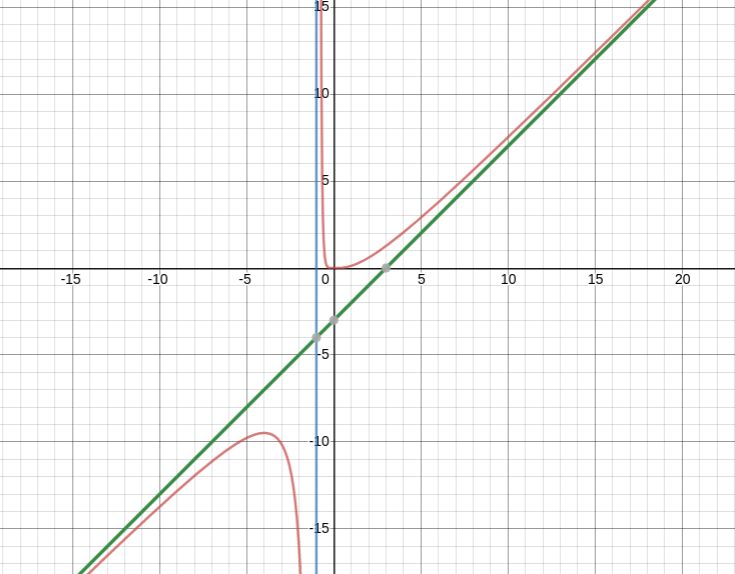
\includegraphics[width=10cm]{img/graf_var4.png}
\end{figure*}

На графике красным обозначена сама функция, а зеленым и синим ее асимптоты.